\documentclass{article}
\usepackage[utf8]{inputenc}
\usepackage{tikz} 
\usepackage{amsmath}
\usetikzlibrary{automata, positioning, arrows}

\title{CS 334 HW1}
\author{Ben Lirio, Liam Keane}
\date{September 10, 2021}

\begin{document}

\maketitle

\section*{Problem 1}
\begin{center}
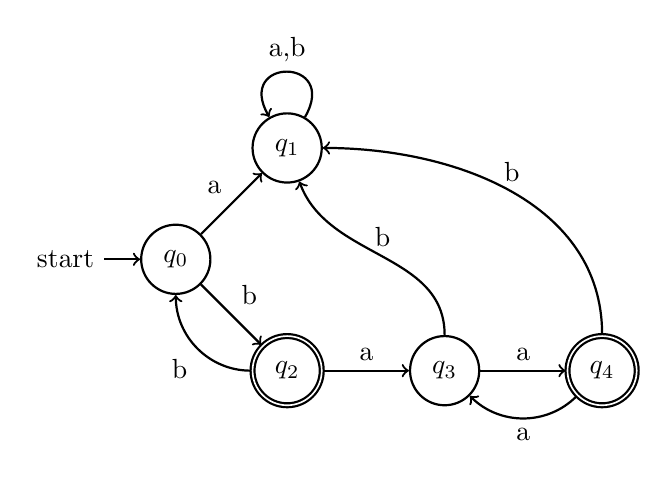
\begin{tikzpicture}[node distance={20mm}, thick, main/.style = {draw, circle}] 
\node[state, initial] (0) {$q_0$}; 
\node[state, above right of=0] (1) {$q_1$};
\node[state, accepting, below right of=0] (2) {$q_2$};
\node[state, right of=2] (3) {$q_3$};
\node[state, accepting, right of=3] (4) {$q_4$};
\draw[->] (0) --node[above right] {b} (2);
\draw[->, out=180, in=270, looseness=1] (2) to node[below left]{b} (0);
\draw[->] (2) --node[above]{a} (3);
\draw[->] (3) --node[above]{a} (4);
\draw[->, out=225, in=315, looseness=1] (4) to node[below]{a} (3);
\draw[->] (0) --node[above left]{a} (1);
\draw[->, out=60, in=120, looseness=5] (1) to node[above]{a,b} (1);
\draw[->, out=90, in=290, looseness =1] (3) to node[above]{b} (1);
\draw[->, out=90, in=0, looseness =1] (4) to node[above]{b} (1);
\end{tikzpicture} 
\end{center}
The above DFA $M$ recognises the language $D$ defined over the alphabet \{$a$,$b$\} as:
\emph{\{w:w contains an even number of a's and an odd number of b's and does not contain the substring ab\}}. 

Within $M$, the state $q_1$ represents what we will call a dead state, there is no way to reach an accept state from it. From the starting state $q_0$, any string that starts with $a$ will go directly to $q_1$ as it is impossible to reach an odd number of $b$'s without containing the string $ab$. 

Strings starting with $b$ will instead move to $q_2$. From $q_2$, a $b$ will move back to $q_0$ as another $b$ is required for the final number of $b$'s to be odd. This is due to the restriction of not containing the string $ab$ making it so that once an $a$ is seen in the input string, no more $b$'s can be added while still being considered valid. The state $q_2$ is also a valid accept state as 0 is an even number of $a$'s.

Upon seeing an $a$ in state $q_2$ the machine moves to state $q_3$. From this point on, any $b$ in the string will result in the substring $ab$ so a $b$ from states $q_3$ or $q_4$ will result in state $q_1$, the "dead state". Between states $q_3$ and $q_4$ is a loop that ensures any time state $q_4$ is reached, there will have been an even number of $a$'s and an odd number of $b$'s making it the second valid accept state in $M$.
\section*{Problem 2}
\subsection*{   2a}
\subsection*{   2b}
\section*{Problem 3}
\subsection*{   3.1}
Given  
\begin{center}
    $A = \{w:\ w\ starts\ with\ an\ a\ and\ has\ at\ most\ one\ b\}$ \\
\end{center}
Find the finite state automata $M$ such that $L(M) = A$.
\begin{center}
    $M = (Q, \Sigma, \delta, q_0, F)$ \\
    $Q = \{q_0,q_1,q_2,q_3\}$ \\
    $\Sigma = \{a,b\}$ \\
    $F = \{q_3\}$
\end{center}
\begin{center}
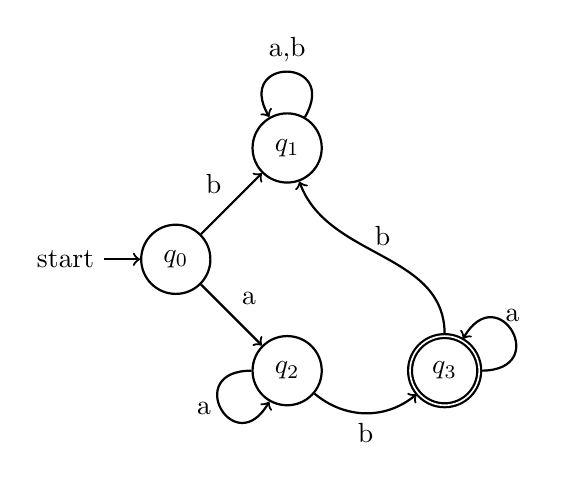
\begin{tikzpicture}[node distance={20mm}, thick, main/.style = {draw, circle}] 
\node[state, initial] (0) {$q_0$}; 
\node[state, above right of=0] (1) {$q_1$};
\node[state, below right of=0] (2) {$q_2$};
\node[state, accepting, right of=2] (3) {$q_3$};

\draw[->] (0) --node[above right] {a} (2);
\draw[->] (0) --node[above left]{b} (1);

\draw[->, out=60, in=120, looseness=5] (1) to node[above]{a,b} (1);

\draw[->, out=180, in=240, looseness=5] (2) to node[left]{a} (2);
\draw[->, out=320, in=220, looseness=1] (2) to node[below]{b} (3);

\draw[->, out=90, in=290, looseness =1] (3) to node[above]{b} (1);
\draw[->, out=0, in=60, looseness=5] (3) to node[above]{a} (3);
\end{tikzpicture} 
\end{center}
\subsection*{   3.2}
\begin{center}
    \begin{tikzpicture}[node distance={15mm}, main/.style={draw, circle}]
        \node[state, initial] (0000) {$q_{0000}$};
        
        \node[state, below of=0000] (0001) {$q_{0001}$};
        \node[state, right of=0001] (0010) {$q_{0010}$};
        \node[state, right of=0010] (0100) {$q_{0100}$};
        \node[state, right of=0100] (1000) {$q_{1000}$};
        
        \node[state, below of=0001] (0011) {$q_{0011}$};
        \node[state, right of=0011] (0101) {$q_{0101}$};
        \node[state, right of=0101] (1001) {$q_{1001}$};
        \node[state, right of=1001] (0110) {$q_{0110}$};
        \node[state, right of=0110] (1010) {$q_{1010}$};
        \node[state, right of=1010] (1100) {$q_{1100}$};
        
        \node[state, below of=0011] (0111) {$q_{0111}$};
        \node[state, right of=0111] (1011) {$q_{1011}$};
        \node[state, right of=1011] (1101) {$q_{1101}$};
        \node[state, right of=1101] (1110) {$q_{1110}$};
        \node[state, below of=0111] (1111) {$q_{1111}$};
        
        \draw[->] (0000) to node[left]{a} (0001)
        \draw[->] (0000) to node[left]{b} (0000)
        \draw[->] (0001) to node[left]{a} (0011)
        \draw[->] (0001) to node[left]{b} (0010)
        \draw[->] (0010) to node[left]{a} (0101)
        \draw[->] (0010) to node[left]{b} (0100)
        \draw[->] (0011) to node[left]{a} (0111)
        \draw[->] (0011) to node[left]{b} (0110)
        \draw[->] (0100) to node[left]{a} (1001)
        \draw[->] (0100) to node[left]{b} (1000)
        \draw[->] (0101) to node[left]{a} (1011)
        \draw[->] (0101) to node[left]{b} (1010)
        \draw[->] (0110) to node[left]{a} (1101)
        \draw[->] (0110) to node[left]{b} (1100)
        \draw[->] (0111) to node[left]{a} (1111)
        \draw[->] (0111) to node[left]{b} (1110)
        \draw[->] (1000) to node[left]{a} (0001)
        \draw[->] (1000) to node[left]{b} (0000)
        \draw[->] (1001) to node[left]{a} (0011)
        \draw[->] (1001) to node[left]{b} (0010)
        \draw[->] (1010) to node[left]{a} (0101)
        \draw[->] (1010) to node[left]{b} (0100)
        \draw[->] (1011) to node[left]{a} (0111)
        \draw[->] (1011) to node[left]{b} (0110)
        \draw[->] (1100) to node[left]{a} (1001)
        \draw[->] (1100) to node[left]{b} (1000)
        \draw[->] (1101) to node[left]{a} (1011)
        \draw[->] (1101) to node[left]{b} (1010)
        \draw[->] (1110) to node[left]{a} (1101)
        \draw[->] (1110) to node[left]{b} (1100)
        \draw[->] (1111) to node[left]{a} (1111)
        \draw[->] (1111) to node[left]{b} (1110)
    \end{tikzpicture}
\end{center}
\section*{Extra Credit}
Let $M_1$ recognize $A_1$, where  $M_1 = (Q_1, \Sigma, \delta_1, q_1, F_1)$, and \\
Let $M_2$ recognize $A_2$, where  $M_2 = (Q_2, \Sigma, \delta_2, q_2, F_2)$

Construct $M$ to recognize $A_1 \bigcup A_2$ 
\end{document}
